\documentclass{beamer}
\usepackage{beamerthemesplit}
\usepackage{wrapfig}
\usepackage{verbatim}
\usetheme{SPbGU}
\usepackage{pdfpages}
\usepackage{amsmath}
\usepackage{cmap} 
\usepackage[T2A]{fontenc} 
\usepackage[utf8]{inputenc}
\usepackage[english,russian]{babel}
\usepackage{indentfirst}
\usepackage{amsmath}
\usepackage{tikz}
\usepackage{multirow}
\usepackage[noend]{algpseudocode}
\usepackage{algorithm}
\usepackage{algorithmicx}
\usetikzlibrary{shapes,arrows}
\usepackage{fancyvrb}
\usepackage{tikz}
\usepackage{pgfplots}
\usepackage{sidecap}
\pgfplotsset{compat=1.9}
\newtheorem{rutheorem}{Теорема}
\newtheorem{ruproof}{Доказательство}
\newtheorem{rudefinition}{Определение}
\newtheorem{rulemma}{Лемма}
\beamertemplatenavigationsymbolsempty

\title[CFPQ with SR]{Context-Free Path Querying with Structural Representation of Result}
% То, что в квадратных скобках, отображается в левом нижнем углу. 
\institute[SPbU]{
    Saint-Petersburg University \\
    Programming Languages and Tools Lab JetBrains}

% То, что в квадратных скобках, отображается в левом нижнем углу.
\author[Semyon Grigorev]{Semyon Grigorev}
\date{July 7, 2017}

\begin{document}
    
    \definecolor{red}{RGB}{255,0,0}
    
    \begin{frame}
        \begin{center}
            {
\includegraphics[width=1.5cm]{pictures/SPbGU_Logo.png}}
        \end{center}
        \titlepage
    \end{frame}
    
    \begin{frame}
        \frametitle{Биоинформатика}
        \begin{itemize}
            \item Множество задач, связанных с обработкой и пониманием биологических данных
            \item Одна из задач --- поиск организмов в метагеномных сборках
        \end{itemize}
    \end{frame}
    
    \begin{frame}
        \frametitle{Геном}
        \begin{itemize}
            \item Геном --- длинная последовательность нуклеотидов
            \item На деле строка над алфавитом \{A, C, G, U\}
        \end{itemize}
    \end{frame}
    
    \begin{frame}
        \frametitle{Получение данных}
        \begin{tabular}{p{5cm} p{7cm}}
            \begin{itemize}
                \item Из биологического материала читаются короткие строчки
                \item Эти кусочки склеиваются в более длинные строки
                \item Множество строчек --- сборка
                \item Данных очень много, поэтому строится граф, сожержащий множество полученных строк
            \end{itemize}
            &
            \begin{figure}[b]
                \centering
                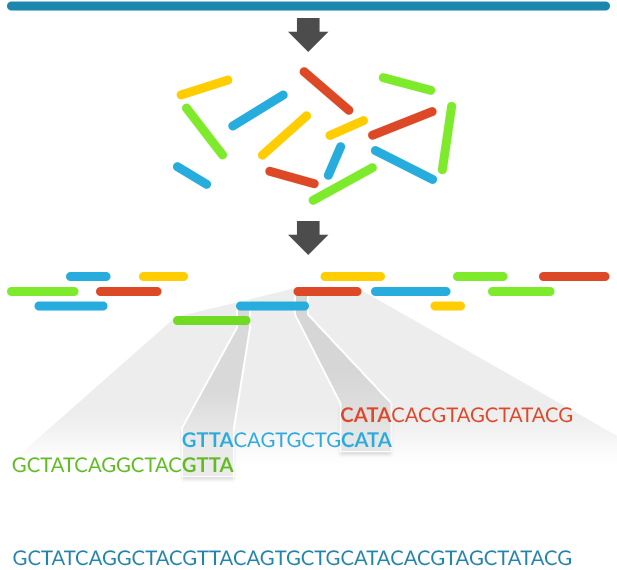
\includegraphics[width=6.5cm]{pictures/readsAssembly.png}  
            \end{figure}
        \end{tabular}
    \end{frame}
    
    \begin{frame}
        \frametitle{Метагеномная сборка}
        \begin{itemize}
            \item Данные из окружающей среды
            \item Изучаем набор генов всех микроорганизмов в образце
        \end{itemize}
    \end{frame}
    
    \begin{frame}
        \frametitle{Что ищем}
        \begin{tabular}{p{6cm} p{5cm}}
            \begin{itemize}
                \item Хочется понять что у нас в сборке
                \item Такие последовательности как тРНК, рРНК позволяют провести классификацию организма
                \item У этих последовательностей есть вторичная структура, которая может быть описана КС-грамматикой
            \end{itemize}
            &
            \begin{figure}[b]
                \centering
                \multirow{-3}*{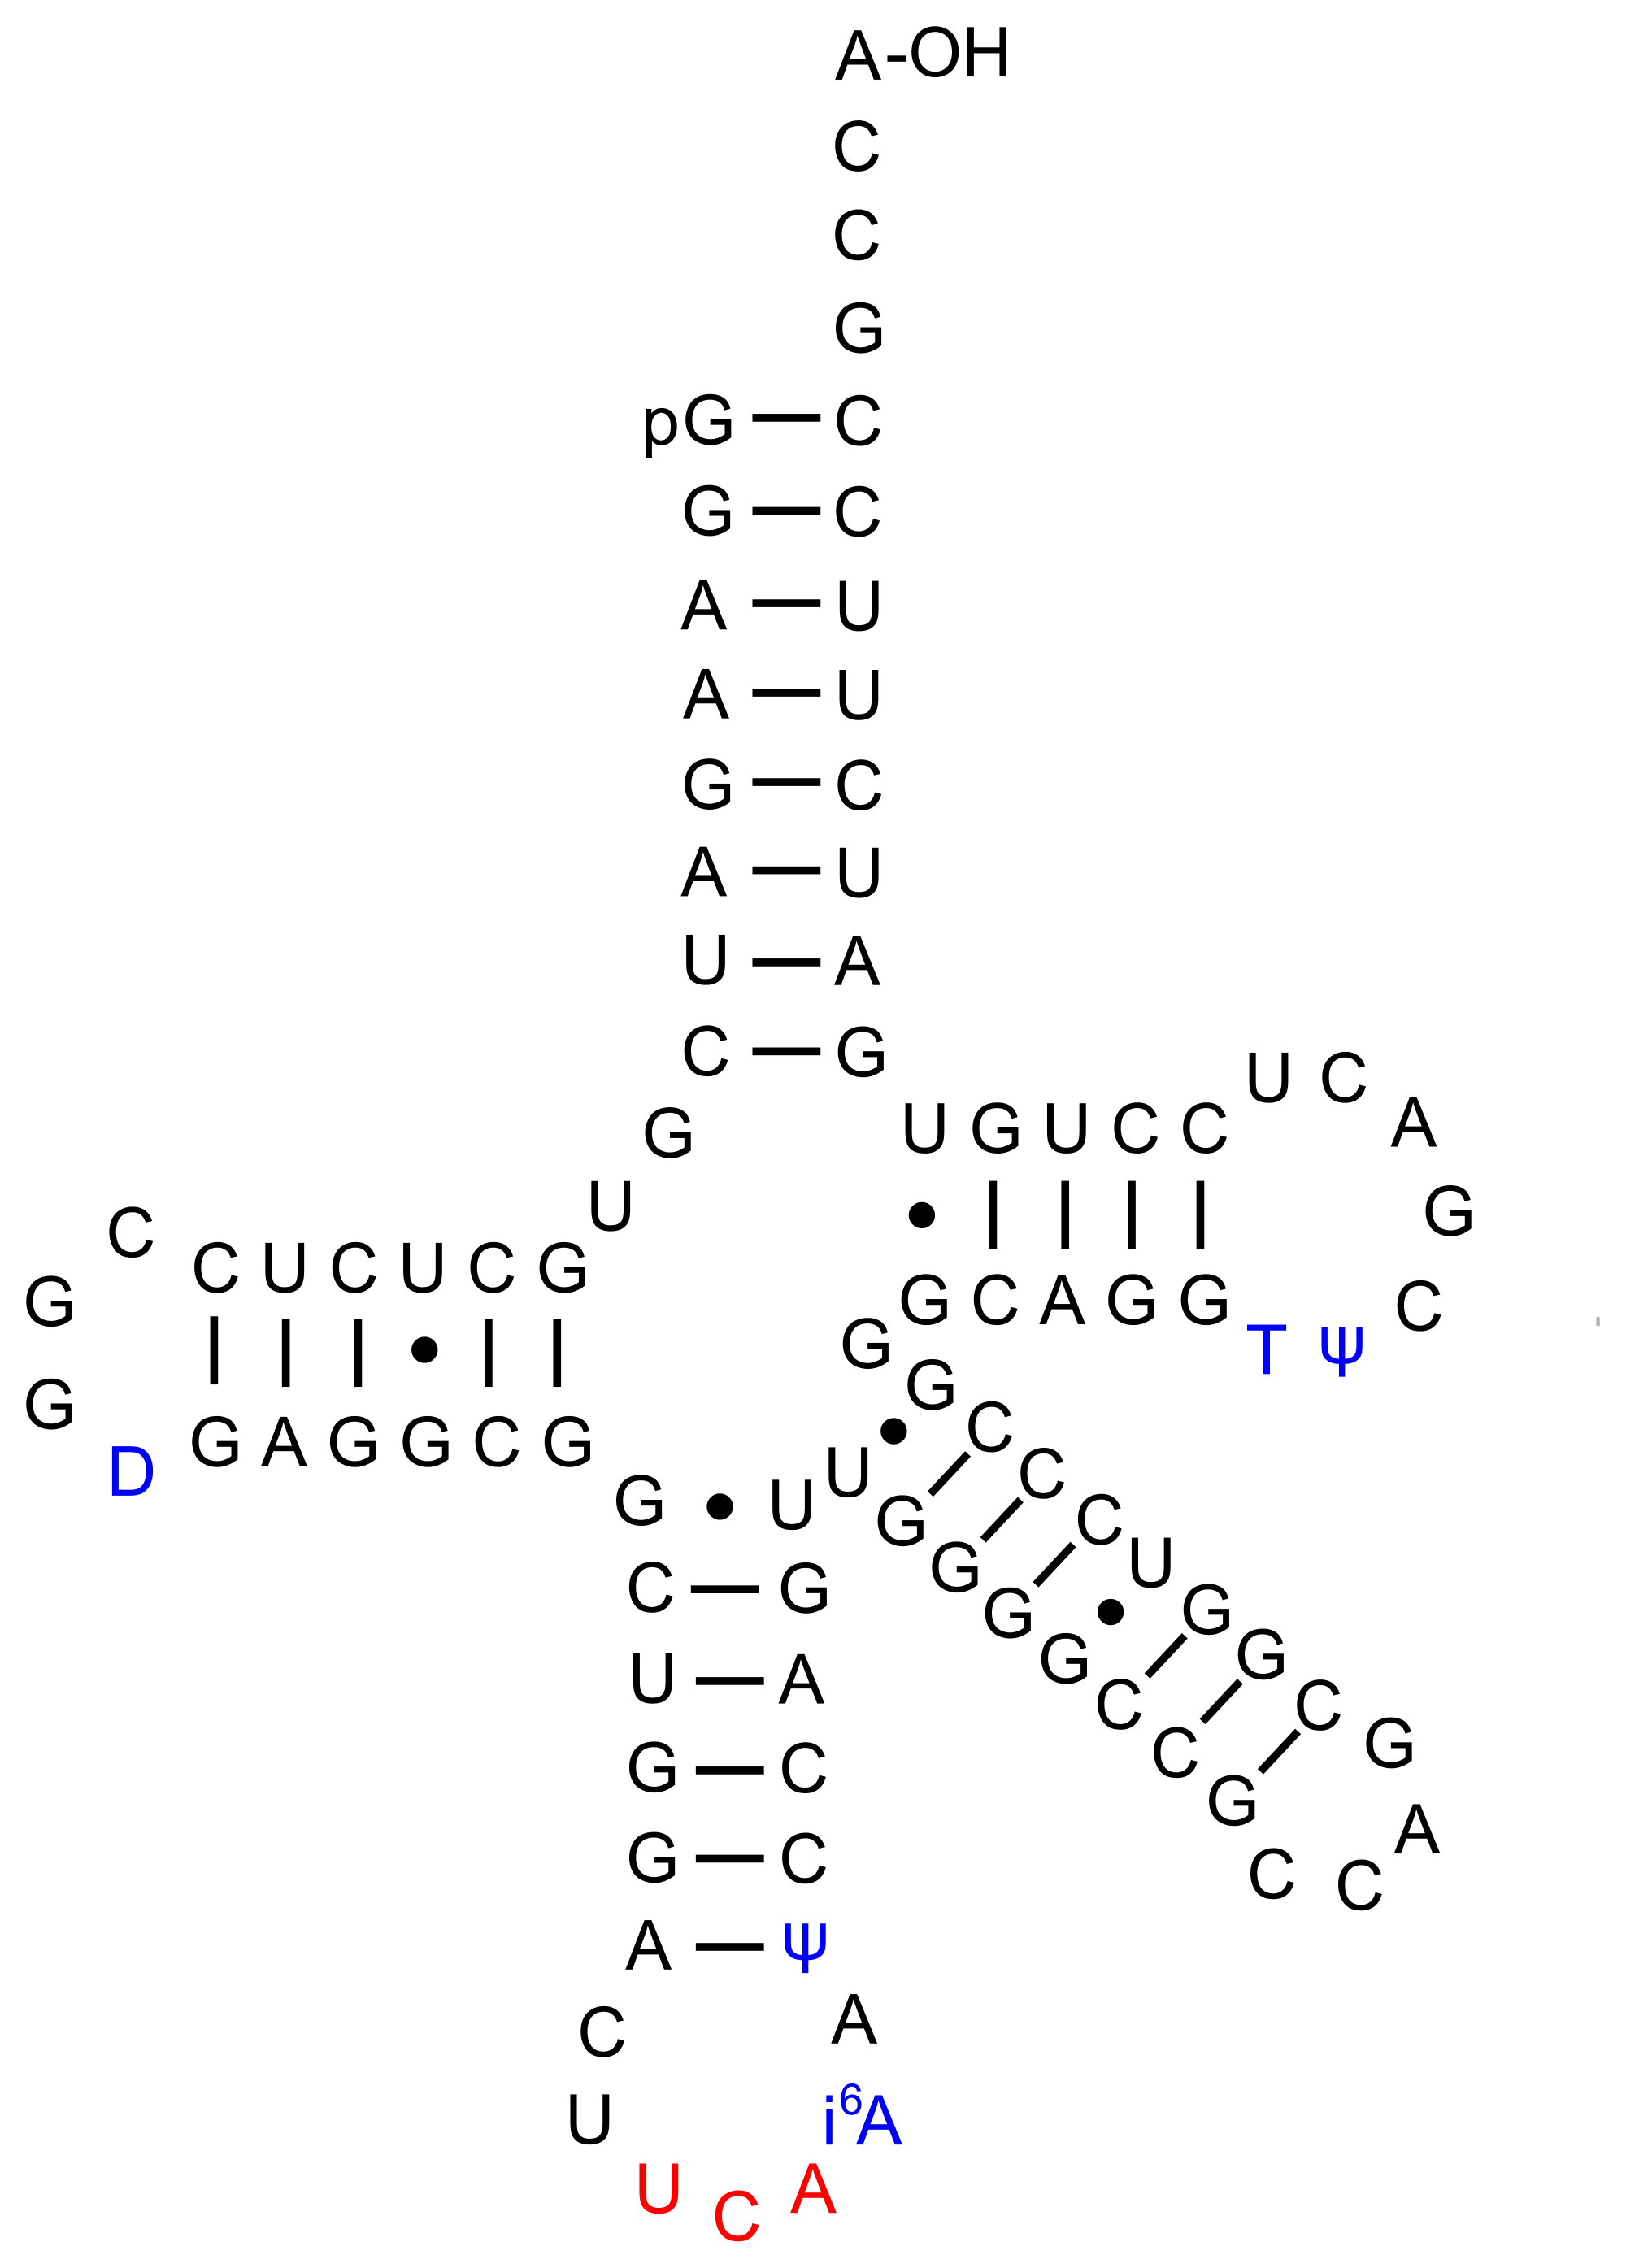
\includegraphics[width=5.2cm]{pictures/TRNA.png}}
                %\multirow{3}*{\caption{Вторичная структура тРНК}}
            \end{figure}
            \\
            $$
            GGAAGAUCG...GCA...  =>
            $$
            &
        \end{tabular}  
    \end{frame}
    
    \begin{frame}
        \frametitle{Грамматика для кусочка тРНК}
        \begin{tabular}{p{6cm} p{5cm}}
            {$\begin{aligned}
                START\ =&\ STEM \\
                STEM\ =&\ a\ STEM\ u \\
                |&\ u\ STEM\ a \\
                |&\ c\ STEM\ g \\
                |&\ g\ STEM\ c \\
                |&\ g\ STEM\ u \\
                |&\ u\ STEM\ g \\
                |&\ ANY^{*}[4..7] \\
                ANY\ =&\ a\ |\ u\ |\ g\ |\ c \\
                \end{aligned}$}
            &
            \multirow{-7}*{
\includegraphics[width=3cm]{pictures/TRNAPart.png}}
        \end{tabular}
    \end{frame}
    
    \begin{frame}
        %\frametitle{Вторичная структура 16s рРНК}
        \begin{tabular}{p{4cm} p{7cm}}
            Вторичная структура 16s рРНК
            &
            \multirow{-7}*{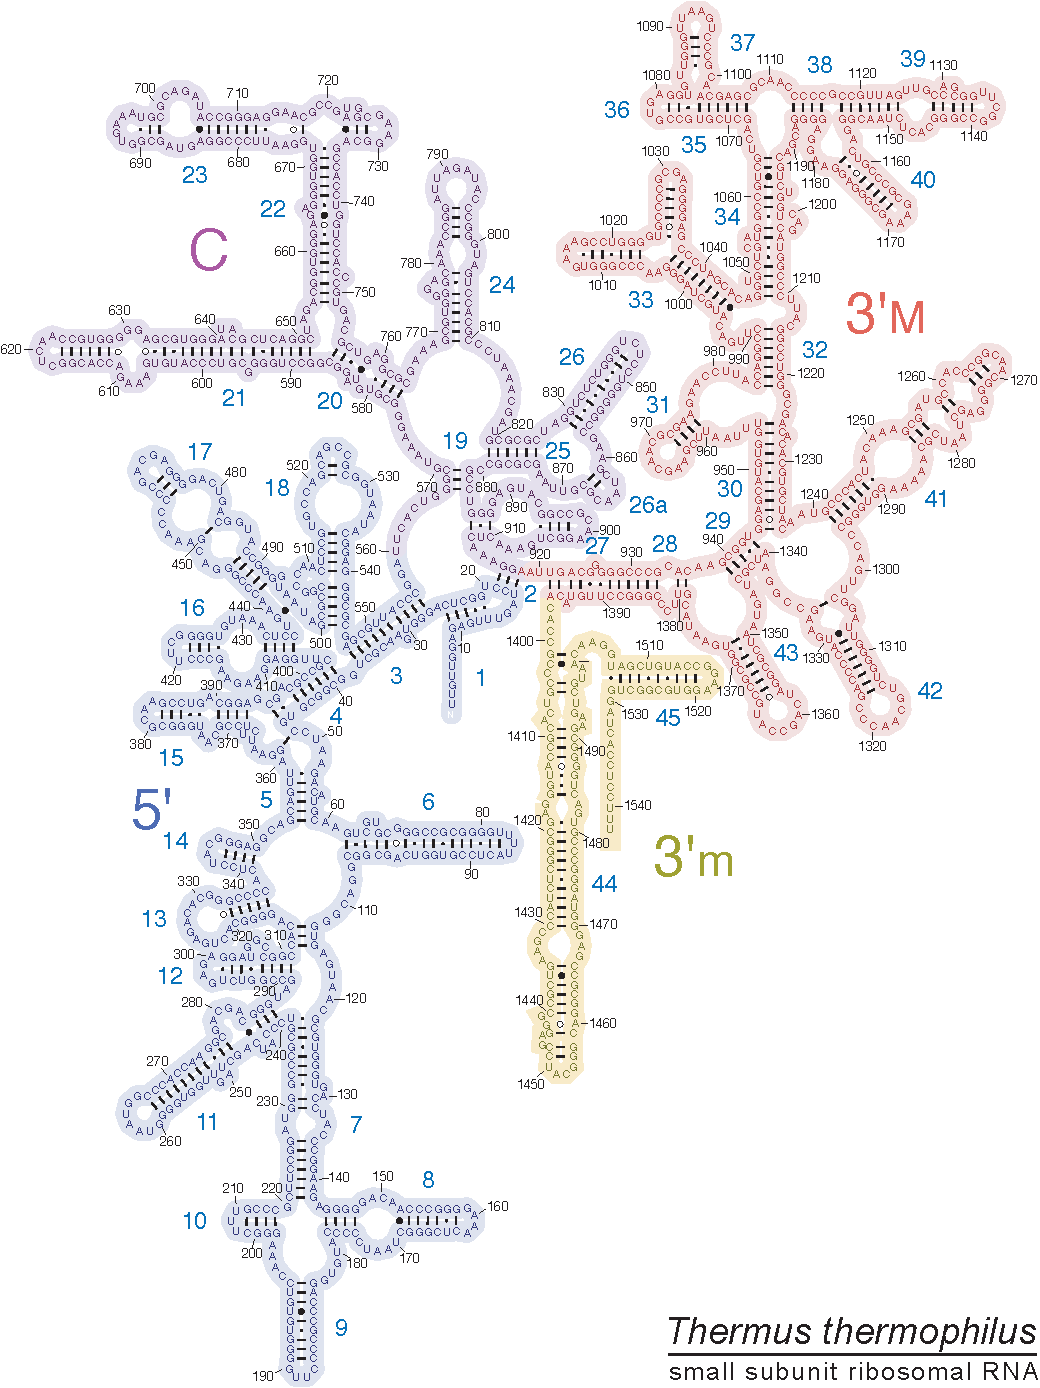
\includegraphics[width=6.5cm]{pictures/thermus_16s_2ndry.pdf}}
        \end{tabular}
    \end{frame}
    
    \begin{frame}
        \frametitle{Graph parsing}
        \begin{itemize}
            \item Задача поиска линейных цепочек, удовлетворяющих КС-грамматике, в графе
        \end{itemize}
    \end{frame}
    
    \begin{frame}
        \frametitle{YaccConstructor}
        \begin{itemize}
            \item В лаборатории созданы алгоритмы
            \item Реализован инструмент, основанный на алгоритме GLL
            \item Умеет решать задачу поиска линейных цепочек в графе, удовлетворяющих КС-грамматике
        \end{itemize}
    \end{frame}
    
    \begin{frame}
        \frametitle{Цель и задачи}
        \textbf{Цель} работы --- научиться классифицировать организмы в метагеномной сборке
        
        \textbf{Задачи}:
        \begin{itemize}
            \item Адаптировать существующий алгоритм под специфику задачи
            \item Провести экспериментальные исследования работы алгоритма
        \end{itemize}
    \end{frame}
    
    \begin{frame}
        \frametitle{GLL}
        \begin{itemize}
            \item Разбор осуществляется при помощи дескрипторов
            \item Дескриптор --- четвёрка (слот, позиция во входе, дерево, вершина стека)
            \item На каждом шаге достаём дескриптор из очереди и разобрав очередной символ создаём новые дескрипторы
        \end{itemize}
    \end{frame}
    
    \begin{frame}
        \frametitle{Подготовка сборки}
        Метагеномные сборки довольно большие, поэтому их необходимо предварительно обрабатывать
        
        
        \begin{itemize}
            \item Infernal позволяет распознавать структуры в линейном входе
            \item Рёбра, длиннее искомых структур можно делить на части и проверять с помощью Infernal
            \item После фильтрации рёбер граф распадается на компоненты связности, на которых алгоритм можно запускать анализатор независимо
        \end{itemize}
    \end{frame}
    
    \begin{frame}
        \frametitle{Отказ от построения дерева}
        \begin{itemize}
            \item Синтаксический анализатор возвращает лишь границы и длину найденных цепочек
            \item Восстановление цепочки идёт путём извлечения подграфа, состоящего из путей заданной длины
            \item Ложные фильтруются с помощью Infernal
        \end{itemize}
        
        \begin{figure}[b]
            \centering
            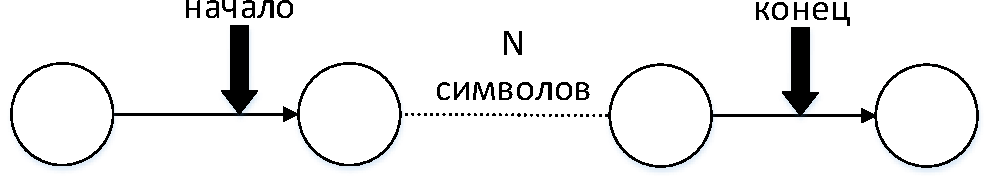
\includegraphics[width=8cm]{pictures/noTree.pdf}  
        \end{figure}
    \end{frame}
    
    \begin{frame}
        \frametitle{Преобразование грамматики}
        \begin{itemize}
            \item Грамматика для 16s рРНК сильно неоднозначная и довольно большая 
            \item Из-за этого количество слотов в грамматике очень много
            \item В процессе разбора создаётся огромное количество дескрипторов 
        \end{itemize} 
    \end{frame}
    
    \begin{frame}
        \frametitle{Преобразование грамматики к автомату}
        \begin{tabular}{p{5cm} p{4cm}}
            Грамматика & Автомат \\
            &   \\
            &   \\
            {$\begin{aligned}
                START\ =&\ STEM \\
                STEM\ =&\ a\ STEM\ u \\
                |&\ u\ STEM\ a \\
                |&\ c\ STEM\ g \\
                |&\ g\ STEM\ c \\
                |&\ g\ STEM\ u \\
                |&\ u\ STEM\ g \\
                |&\ ANY^{*}[3..6] \\
                ANY\ =&\ a\ |\ u\ |\ g\ |\ c \\
                \end{aligned}$}
            &
            \multirow{-8}*{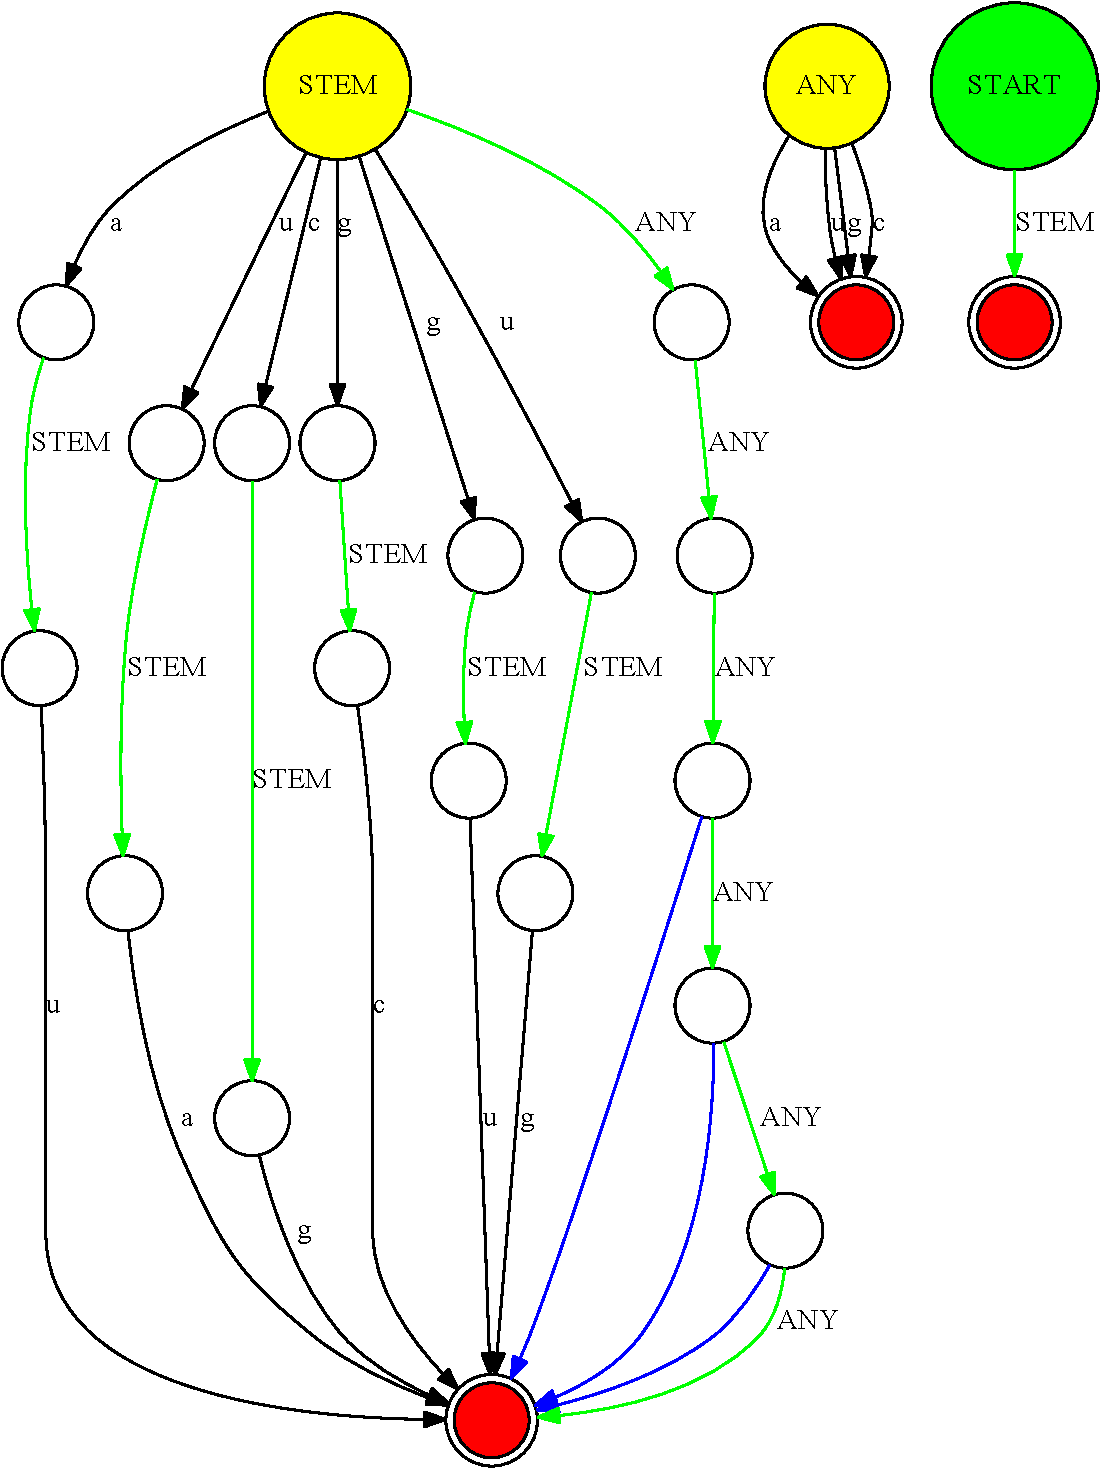
\includegraphics[height=7cm]{pictures/initialNFA.pdf}}
        \end{tabular}
    \end{frame}
    
    \begin{frame}
        \frametitle{Минимизация автомата}
        \begin{tabular}{p{6cm} p{5.5cm}}
            Изначальный автомат & Минимизированый автомат \\
            &   \\
            &   \\
            &   \\
            &   \\
            &   \\
            &   \\
            &   \\
            &   \\
            &   \\
            &   \\
            &   \\
            &   \\
            \multirow{-13}*{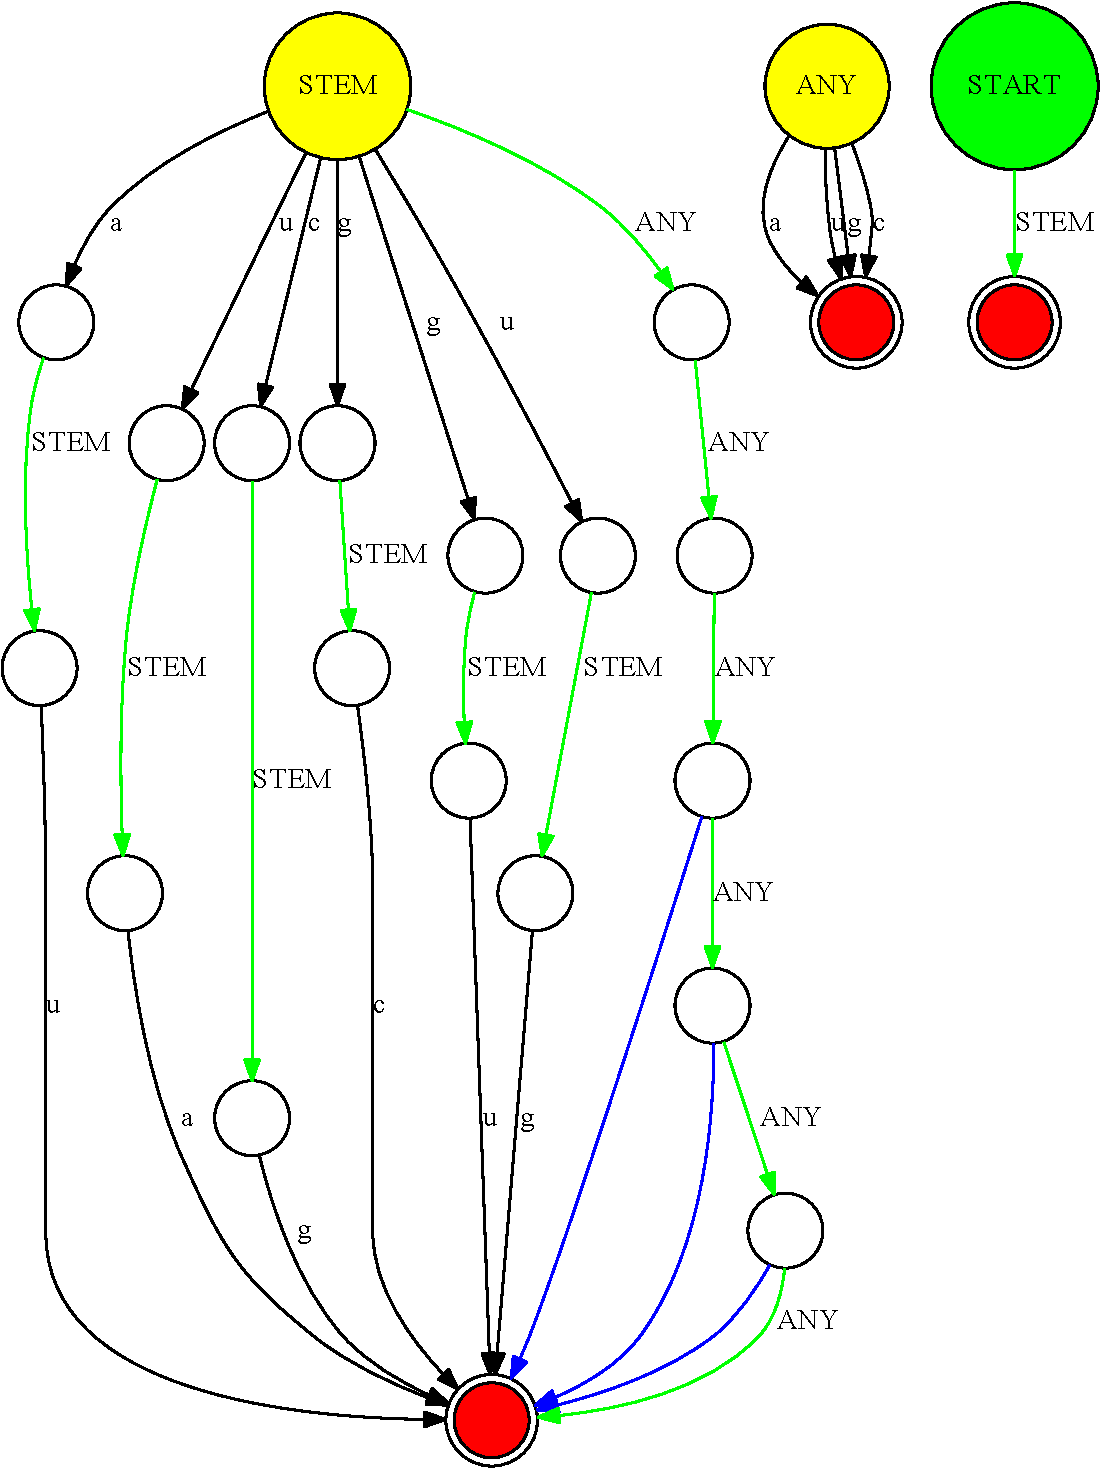
\includegraphics[height=7cm]{pictures/initialNFA.pdf}}
            &
            \multirow{-13}*{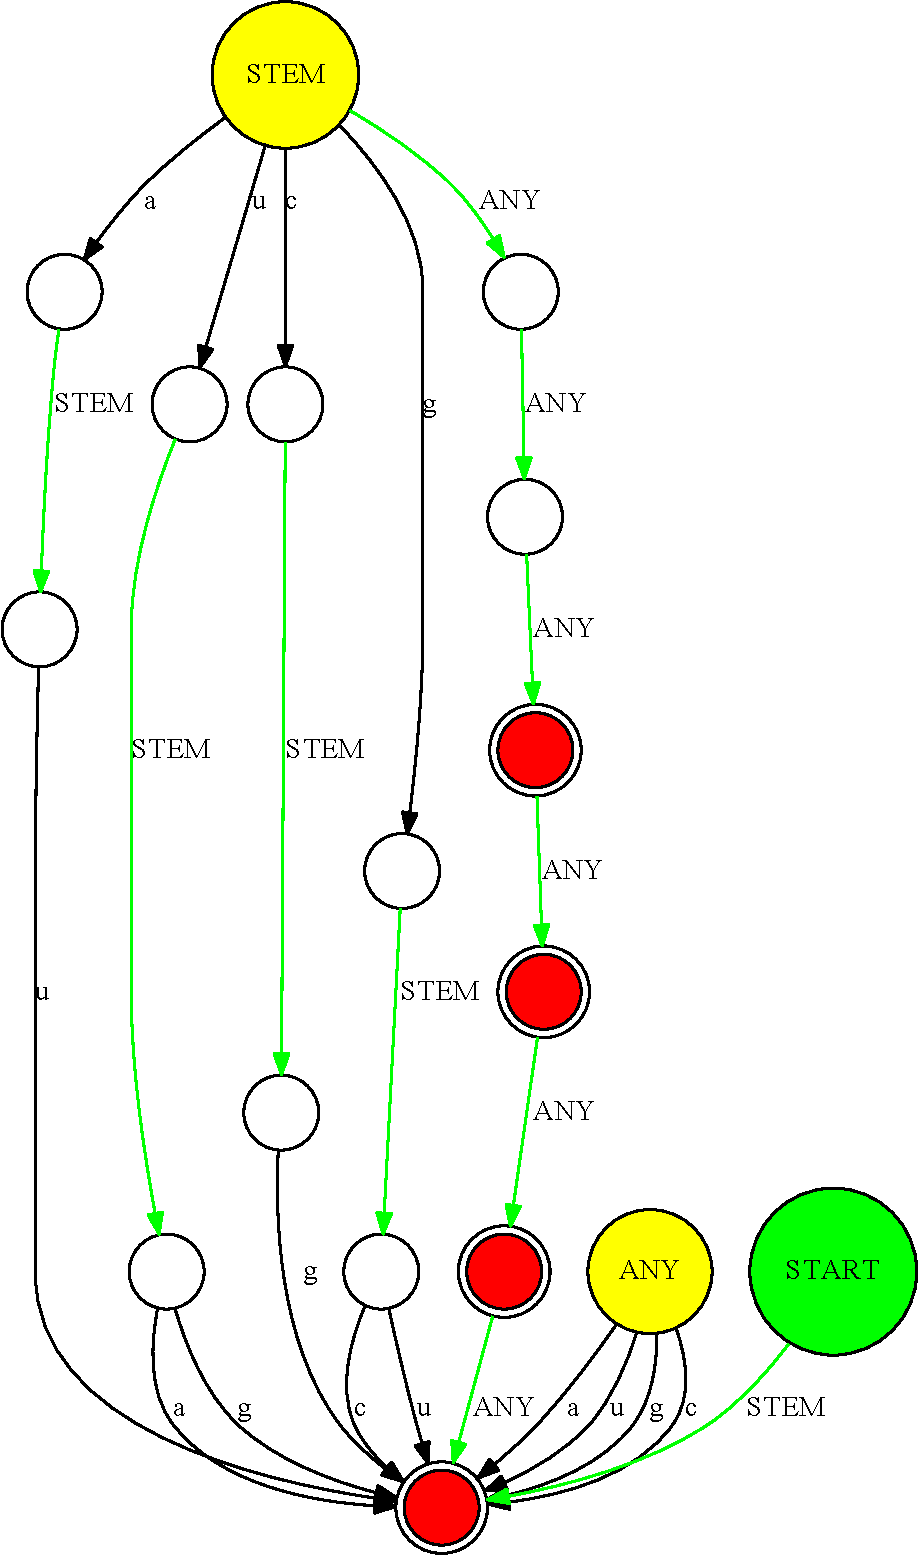
\includegraphics[height=7cm]{pictures/minimizedDFA.pdf}}
        \end{tabular}
    \end{frame}
    
    \begin{frame}
        \frametitle{Эксперименты}
        Результаты работы на сборке, состоящей из 59000 вершин и 87000 рёбер
        и грамматике кусочка 16s рРНК, длиной около 300 символов
        \begin{center}
            \begin{tabular}{ p{2.5cm} | p{2cm} | p{2.5cm}}
                & начальная грамматика & мин. автомат \\ \hline
                Время работы                & 10 ч.                & 3 ч. 40 мин. \\ \hline
                Кол-во слотов /состояний    & 41                   & 17           \\ \hline
            \end{tabular}
        \end{center}
        Эксперименты проводились на машине с 32 ГБ RAM и CPU core i7-4790
    \end{frame}
    
\begin{frame}
\frametitle{Направление работ}
    \begin{figure}%[ht]
   \begin{center}
   \centering
   \begin{subfigure}[b]{0.4\textwidth}
   \[
\begin{array}{rl}
   0: & S \rightarrow \text{\textit{subClassOf}}^{-1} \ S \ \text{\textit{subClassOf}} \\ 
   1: & S \rightarrow \text{\textit{type}}^{-1} \ S \ \text{\textit{type}} \\ 
   2: & S \rightarrow \text{\textit{subClassOf}}^{-1} \ \text{\textit{subClassOf}} \\ 
   3: & S \rightarrow \text{\textit{type}}^{-1} \ \text{\textit{type}} \\ 
\end{array}
\]
   \caption{Grammar for query 1}
   \label{grammarQ1}
   \end{subfigure}
   \hspace{2em}
   \begin{subfigure}[b]{0.4\textwidth}
   \[
\begin{array}{rl}
   0: & S \rightarrow B \ \text{\textit{subClassOf}} \\ 
   0: & S \rightarrow \text{\textit{subClassOf}} \\ 
   1: & B \rightarrow \text{\textit{subClassOf}}^{-1} \ B \ \text{\textit{subClassOf}} \\
   2: & B \rightarrow \text{\textit{subClassOf}}^{-1} \ \text{\textit{subClassOf}} \\ 
\end{array}
\]
   \caption{Grammar for query 2}
   \label{grammarQ2}        
   \end{subfigure}
   \end{center}
   \caption{Grammars for evaluation}
    \label{GrammarsForEvaluation}
\end{figure}
\end{frame}
    
\begin{frame}
        \frametitle{Направление работ}
\begin{table}[t]
\centering
\caption{Evaluation results for Query 1 and Query 2}
\label{tbl1}

\begin{tabular}{ | c | c | c | c | c | c |}
\hline
Ontology & \#triples & \multicolumn{2}{|c|}{Query 1} & \multicolumn{2}{|c|}{Query 2} \\
\cline{3-6}
& & time(ms) & \#results & time(ms) & \#results \\
\hline 
\hline
skos        & 252 & 10 & 810 & 1 & 1 \\
generations & 273 & 19 & 2164 & 1 & 0 \\
travel      & 277 & 24 & 2499 & 1 & 63 \\
univ-bench  & 293 & 25 & 2540 & 11 & 81 \\
foaf        & 631 & 39 & 4118 & 2 & 10 \\
people-pets & 640 & 89 & 9472 & 3 & 37 \\
funding     & 1086 & 212 & 17634 & 23 & 1158 \\
atom-primitive & 425 & 255 & 15454 & 66 & 122 \\
biomedical-measure-primitive & 459 & 261 & 15156 & 45 & 2871 \\
pizza       & 1980 & 697 & 56195 & 29 & 1262 \\
wine        & 1839 & 819 & 66572 & 8 & 133 \\
\hline
\end{tabular}

\end{table}
    \end{frame}
\end{document}